\documentclass[preprint,12pt]{elsarticle}
\usepackage{amsmath,amssymb}
\usepackage{booktabs}
\usepackage{tabularx}
\usepackage{multirow}
\usepackage{graphicx}
\usepackage{xeCJK}
\setCJKmainfont{Noto Serif CJK SC}
\usepackage[hidelinks]{hyperref}
\setlength{\emergencystretch}{3em}
\journal{Nuclear Engineering and Technology}

\begin{document}

\begin{frontmatter}
\title{KnowledgeNexus: A Traceable Graph--Vector Knowledge Infrastructure and
Adaptive Multi-Channel Retrieval for Nuclear Science Literature}
\author[addr1]{Zhiqian Chen\corref{cor1}}
\ead{chenzhiqian@cdut.edu.cn}
\cortext[cor1]{Corresponding author.}
\address[addr1]{Chengdu University of Technology, Chengdu, China}

\begin{abstract}
Nuclear-science organisations face a rapidly growing, heterogeneous literature
base with no domain-adapted retrieval infrastructure. We present
KnowledgeNexus, a knowledge-centre platform that (i) constructs a traceable
corpus of nuclear science literature with dictionary-driven entity curation,
typed-relation enrichment and bilingual aliases; (ii) retrieves through an
adaptive fusion of five channels---lexical, dense, synthetic-query, entity
co-occurrence and doc-level bibliography vectors---gated by query intent; and
(iii) is evaluated with an honest-ablation methodology on self-generated,
corpus-first question sets across four disciplines (27--3{,}479 documents) and
three public multi-hop benchmarks against BM25, LlamaIndex, HippoRAG~2 and
LightRAG baselines under identical corpora, embedders and question sets. At
full-corpus scale the system attains coverage@10 of 0.669 versus 0.351 for a
dense-RAG baseline (LlamaIndex; 1.3\,s vs 35.9\,s per query, the latter a
brute-force scan over its 37\,GB vector store), and intent-gated
channel weighting lifts real-user query hit@10 from 0.897 to 0.949; a
query-time LLM pipeline
(rewrite$\to$fuse$\to$rerank) wins association coverage@10 (+10.1pt,
CI-significant) but only at ${\sim}$60$\times$ latency and zero asset
accumulation, tracing the capability-versus-infrastructure trade-off. We report negative results (a
reranker, doc caps, static weights, and a production incident in which a
category-word schema lexicon collapsed 61{,}137 documents onto 575 type-level
entities---diagnosed, repaired with a 3{,}702-term corpus-attested lexicon,
and rebuilt to 1{,}871 entities with a functioning relation layer) and
engineering findings (filtered-HNSW robustness, write-window rank jitter, a
silently row-swallowing \texttt{INSERT IGNORE}) with the same rigour as
positive ones. Corpus, question sets, evaluation harness and reproduction
commands are released.
\end{abstract}

\begin{keyword}
nuclear science literature \sep domain knowledge base \sep multi-channel
retrieval \sep entity enrichment \sep corpus-first benchmark \sep honest
ablation
\end{keyword}
\end{frontmatter}

\section{Introduction}
\label{sec:intro}

Nuclear-domain literature intelligence is a demanding consumer of retrieval
infrastructure. Its corpus spans regulatory and academic sources, is dense
with specialized terminology, is bilingual (Chinese regulatory texts against
English journal literature), and---because conclusions feed safety-relevant
analyses---carries an \emph{evidence-traceability} requirement: every
retrieved fact must anchor to a specific passage in a specific document. A
generic vector store answers; it does not anchor, disambiguate bilingual
terms, or reason over domain entities.

Existing options each miss a layer. General-purpose RAG frameworks (dense
retrieval plus optional reranking) ship no domain entity infrastructure at
all; graph-RAG systems build one, but their construction cost grows
super-linearly with corpus scale---our measurements put LightRAG at $>$13\,h
for 82 documents, infeasible for an 80-thousand-document library
(Section~\ref{sec:results}). Domain-adapted encoders presuppose exactly the
entity-and-evidence substrate they would index. And the field lacks
domain-generated benchmarks: evaluation practices borrow general web queries
whose answer distribution says nothing about bilingual regulatory--academic
retrieval.

We present KnowledgeNexus (KNC), a knowledge-infrastructure-first platform
for nuclear science literature, and report its construction, retrieval, and
evaluation end to end at production scale (80{,}852 documents, 7.2M chunks).
Our contributions are fourfold. (i)~A \emph{traceable construction
pipeline}---schema-driven, dictionary-based entity enrichment with
LLM-adjudicated typed relations, every claim anchored to chunk-level
evidence---whose retrieval-facing value, our channel ablations show, runs
through asset supply (bilingual aliases into the lexical channel, reranker
context and knowledge chains into the deep lane and generation) rather
than through fusion votes, a decomposition we state up front and quantify
in Section~\ref{sec:results}. (ii)~A \emph{five-channel, intent-gated retrieval architecture}
(lexical, dense, doc-vector, co-occurrence, graph) fused by weighted
reciprocal-rank fusion (RRF) with query-type-adaptive gating, plus a deep
track for budget-rich consumers. (iii)~A \emph{corpus-first benchmark
methodology}---question sets generated from and scoped to the actual library,
evaluated by paired-bootstrap coverage/recall with system-level attribution
made explicit. (iv)~An \emph{honest engineering record}: negative results and
production incidents are reported with the same rigour as positive ones.

Headline results: on the nuclear-electronics corpus, full-library associative
retrieval reaches any-hit@10 of 1.000 with coverage@10 of 0.652 and p50
latency 1.46\,s---versus a dense baseline that loses a third of its any-hit
by 16$\times$ corpus growth; construction costs 1--2 orders of magnitude less
than graph-RAG alternatives; and the architecture transfers across four
disciplines at R@10~$\geq$~0.90.

\section{Related Work}
\label{sec:related}

Nuclear-domain NLP falls into three strands. \textbf{Regulatory-side
systems} (RADIANT-LLM~\cite{radiantllm}) adapt generic QA stacks to nuclear
regulatory corpora; they demonstrate domain need but inherit the vector-store
substrate, without entity layers or evidence anchoring. \textbf{Domain
pretraining} (NukeLM~\cite{nukelm}) and ontology-grounded small-scale systems
(CurieLM~\cite{curielm}) adapt encoders or curate ontologies for narrow
collections; neither scales to tens of thousands of full-text documents, and
both presuppose the infrastructure they would need.
Fayyaz et al.'s survey~\cite{fayyaz} names three challenges---terminology
density, bilingual sources, traceability---which our architecture answers
channel by channel (dictionary-driven entity enrichment; bilingual alias
expansion in the lexical channel; evidence-anchored citations in every
retrieved chunk). HydroLLM-Benchmark~\cite{hydrollm} is precedent for
domain-generated benchmarks; ours extends the practice with paired-bootstrap
significance and corpus-scoped arms. In the \textbf{graph-RAG lineage},
HippoRAG~\cite{hipporag}, LightRAG~\cite{lightrag} and
GraphRAG~\cite{graphrag} demonstrate multi-hop or global-sensemaking gains
at small-to-moderate scale, and RAPTOR~\cite{raptor} represents the
parallel hierarchical-summarization line; our measurements
(Section~\ref{sec:results}) show their
construction cost super-linear and their LLM-extracted entities fragile on
domain full text (10.6\% chunk-NER failure versus 0.25\% on Wikipedia-grade
text). In the \textbf{query/document-expansion lineage},
doc2query~\cite{doc2query} and HyDE~\cite{hyde} transform one side of the
match into the other's space; our synq channel is a doc2query asset built
at ingestion, and our deep-lane HyDE experiment (Section~\ref{sec:results})
is a trained-rewriter slot that the training-free variant could not fill.
The differentiation, in one sentence: prior work either adapts generic
frameworks to nuclear QA or pretrains domain encoders; none builds the
knowledge-infrastructure layer---entities, typed relations, bilingual
aliases, evidence anchoring---nor evaluates it with domain-generated,
corpus-first benchmarks at production scale.

\section{System Overview}
\label{sec:system}

\subsection{Architecture}

KnowledgeNexus organises the platform as four cooperating services over a
single authoritative data plane: an ingestion worker, an enrichment worker, a
retrieval API, and an administration/observer pair. All persisted state lives
in three authority stores---MySQL for bibliographic and entity registries,
OpenSearch for chunk/document/query/entity projections with kNN indexes, and
MinIO for raw artefacts---accessed exclusively through service interfaces
(Fig.~\ref{fig:arch}). Three properties matter for the rest of this paper:

\begin{figure}[t]
\centering
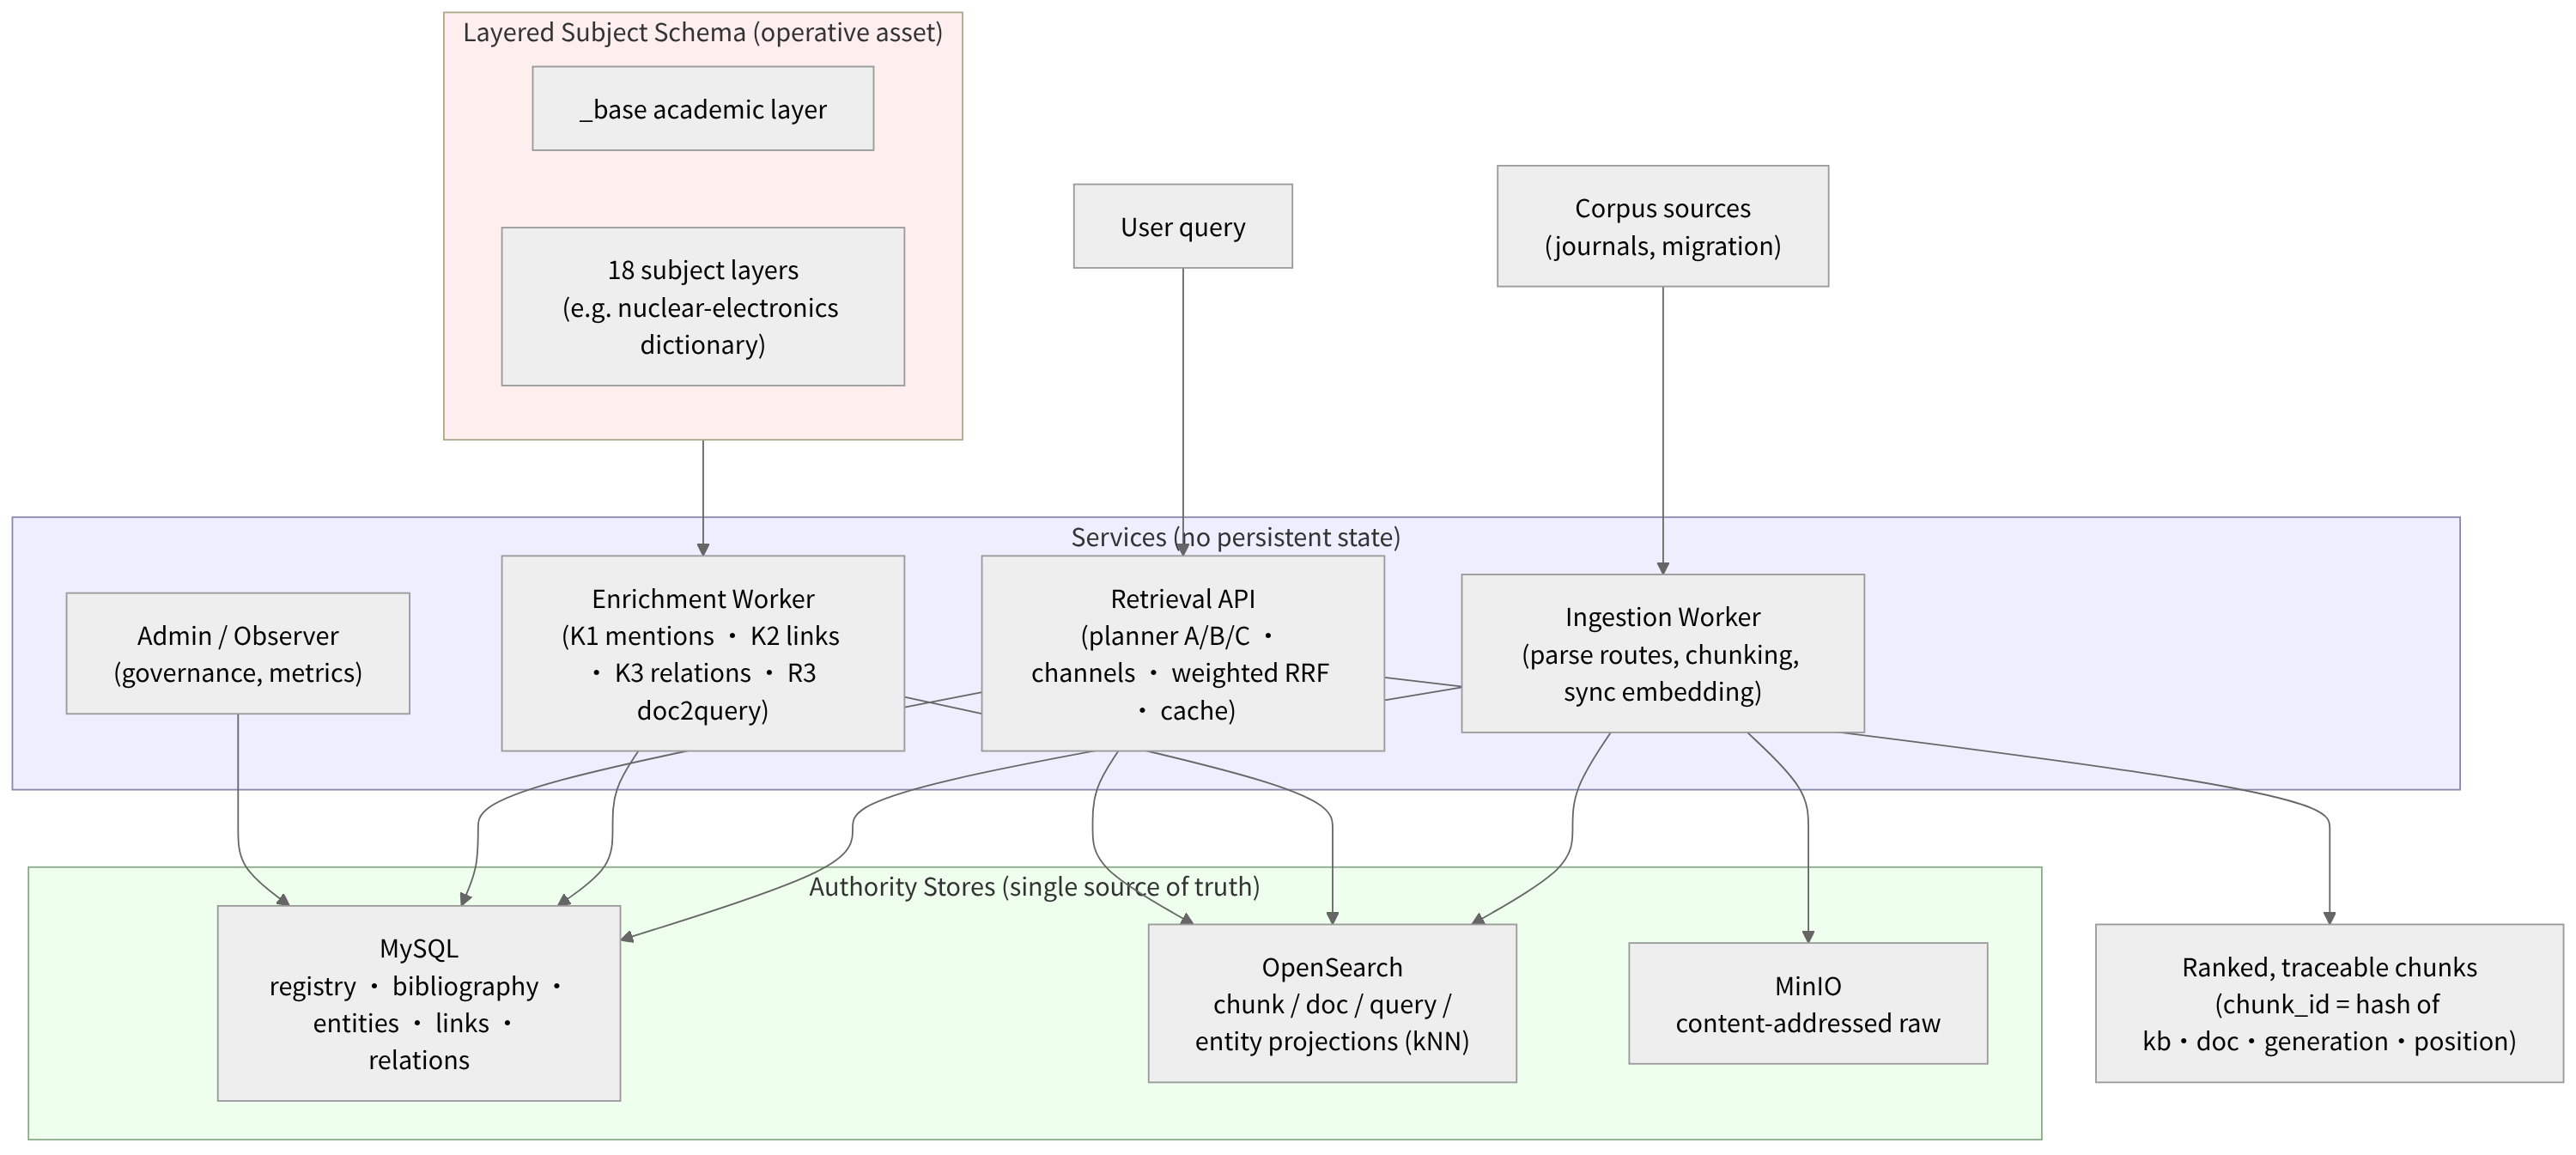
\includegraphics[width=0.92\textwidth]{fig1.png}
\caption{System overview: four services over an authoritative data plane.}
\label{fig:arch}
\end{figure}

\textbf{(a) Data authority.} Chunk text exists only in the search projection;
MySQL \texttt{kb\_chunks} stores spans, and \texttt{chunk\_id} is a
deterministic hash of (kb, doc, generation, position), so every retrieved
passage is traceable to its source span, parse generation and chunker
version. Documents ingested through the batch endpoint are fingerprinted
(content-addressed raw store + \texttt{stable\_fingerprint} uniqueness),
making ingestion idempotent and auditable.

\textbf{(b) Discipline schemas.} Each knowledge base binds a layered subject
schema (\texttt{\_base} academic layer + 18 subject layers + custom layers).
The schema is not documentation but an operative asset: its term dictionary
drives mention extraction (K1), its entity/relation types drive linking and
typed-relation adjudication (K2/K3). We show in Section~\ref{sec:results}
that schema binding is the root of the entity channel: a test corpus bound to
the generic schema yields 14 canonical entities where the
nuclear-electronics schema yields 1{,}166.

\textbf{(c) Capability bits.} Every enriched channel is guarded by a
per-partition capability bit consulted at query time; a channel whose data is
absent or stale degrades silently. This is what allows the honest-ablation
methodology of Sections~\ref{sec:channels}--\ref{sec:results}: channels can
be switched on/off per query without reindexing.

\subsection{Retrieval planner}

Retrieval is a planner over channels (strategy A single-KB direct, B
bibliography drill-down, C federation; topic routing D/E experimental).
Channels contribute ranked chunk lists fused by weighted reciprocal-rank
fusion (RRF) with per-channel weights; the intent gate (template words +
$\geq$2 dictionary entity surfaces in the query) modulates weights for
association-intent queries. Latency-critical paths are cached with an ACL- and
channel-set-aware key; configuration changes (weights, caps) deliberately
invalidate nothing and require an explicit cache purge---an operational
discipline documented after it bit us twice.

\section{Traceable Construction}
\label{sec:construction}

\subsection{Corpus and ingestion}

\textbf{Corpus status.} The full-window ingestion completed: 80{,}855
documents parsed from 75{,}476 source PDFs (80{,}852 ACTIVE) across
nuclear-domain journals---the English library led by Sensors (21.4k), JHEP
(13.1k), Phys.\ Rev.\ D (6.2k) and Phys.\ Lett.\ B, the Chinese library by
原子能科学技术, 强激光与粒子束, 核动力工程 and 核电子学与探测技术---across
13 active knowledge bases and 7{,}229{,}225 text chunks, with figure-media
backfill closing at 100\% \texttt{media\_uri} coverage. Ingestion accepts
parsed Markdown (MinerU route) or pre-chunked text (RADAI migration route)
and produces chunks at ${\sim}1{,}200$ characters respecting heading
structure, tables as standalone blocks, with title-context prefixes. Chunk
vectors (Qwen3-Embedding-8B, 4{,}096-d)~\cite{qwen3emb} are written
synchronously with ingestion; lexical and dense channels are therefore
immediately queryable while enrichment proceeds asynchronously.

\subsection{Enrichment pipeline (K1--K3)}

\textbf{K1 mentions} are dictionary-and-rule scans of chunk text against the
bound schema's term dictionary (plus bilingual aliases), persisted in
\texttt{raw\_mention} with stable mention ids---no LLM calls. \textbf{K2
linking} resolves mentions to canonical entities via alias tables and, only
for ambiguous surfaces, a context disambiguation LLM call. \textbf{K3 typed
relations} mines co-occurrence candidate pairs and adjudicates relation types
with the LLM, persisting typed edges with evidence. Doc2query synthesis (R3)
generates synthetic queries per chunk (${\sim}3$ per chunk,
doc2query-style document expansion~\cite{doc2query}) into a query
index consumed by the synq channel; doc/topic summaries feed the bibliography
and abstract vectors.

\textbf{Model configuration, for reproducibility.} All pipeline LLM calls
(doc2query synthesis, relation adjudication, context disambiguation,
question phrasing) use Qwen3.6-35B-A3B (AWQ 4-bit quantization) served
with vLLM behind a round-robin router over seven GPUs. The endpoint
exposes it under the served-model alias \texttt{qwen3.5-35b}, which
predates the current weights---the version numbers genuinely differ
between alias and weights; the deployed model is the 3.6 weights.
Embeddings are Qwen3-Embedding-8B---native 4{,}096-d,
Matryoshka-truncated to 1{,}024 \textbf{on both the index and the query
side} (the deployed kNN indexes store 1{,}024-d vectors; the truncation
was adopted after an ablation measured zero fusion-level change). The
deep-lane cross-encoder reranker is Qwen3-Reranker-4B for every
experiment dated through 2026-10-04---including the hard-set component
separation (Section~\ref{sec:autopsy}) and the deep-lane adoption
bundle---and OneJev-4B (OmniJev's public vLLM release on Hugging Face)
for the 2026-10-05 production validation whose numbers appear alongside
that date. The closed-book control of Section~\ref{sec:bench} uses the
same 35B pipeline LLM (temperature 0); a stronger closed-book model would
make that control stricter, and we did not run one.

\textbf{Cost profile.} For a 300-document nuclear slice (29.6M characters),
full enrichment ${\approx}$1\,h dominated by 18{,}454 doc2query LLM calls at
concurrency 70; dictionary stages are negligible. This contrasts with
graph-RAG construction over the same corpus: HippoRAG~2 required 4.1\,h and
LightRAG did not finish within 7\,h on an 82-document subset (serial entity
merge, superlinear in graph size)---a scale wall we report as a finding.

\subsection{Governance}

Entity assets mutate only through a four-stage governance loop---\emph{scan}
(vector-neighbour and name-containment candidate generation, with a type
guard), \emph{adjudicate} (conservative LLM rulings; a FLIP is accepted only
when the self-reported direction and the label agree, otherwise the pair is
downgraded to KEEP), \emph{merge} (reversible batches recorded in
\texttt{merge\_log} with score, rationale, and before/after snapshots; link
endpoints are redirected so \texttt{link\_id} survives), and \emph{replay}
(reverse-order rollback restoring MySQL and the graph store consistently).
Every mutation is thus auditable and reversible by construction.

Three measured outcomes anchor the governance claim:

\begin{enumerate}
\item \textbf{The LLM adjudicator failed its own pre-registered gate.} The
formal acceptance gate (merge precision $\geq$96\%, effective dedup rate
$\geq$50\%) was evaluated for the first time on the full nine-library corpus
after the scan stage gained an OpenSearch kNN path (pure-Python candidate
generation is $O(n^2)$---350M pairs at 26.6k entities---and had silently
kept the gate from ever being evaluated). LLM adjudication accepted 115
candidate pairs; an independent review of a 50-pair sample found 5
errors---precision 90.0\%~$<$~96\%, so automatic merging remains disabled.
(Rejected pairs: 20 sampled, 0 misses.) The failure modes are systematic, not
random: corporate legal-entity suffixes (Wiley Ltd/Inc), section titles
versus teaching-point variants, and near-synonym facilities (injection versus
recharge wells).

\item \textbf{Deterministic rules cleared the actual duplicate population.}
The gate run surfaced 87 same-name, same-type multi-ACTIVE groups---all
person entities, all parser accent variants (Nicol\`o/Nicolo/Nicol\'o,
Lef\`evre/Lefevre). Unicode NFD folding grouped 85 groups/90 pairs, plus 2
pairs of \L{} (no NFD decomposition): 92 pairs merged with zero LLM
involvement, in 19 reversible batches. Ledger reconciliation was exact
(ACTIVE 34{,}563$\to$34{,}471; MERGED 667$\to$759) and retrieval showed zero
regression (R@10 0.9722, MRR 0.831 unchanged).

\item \textbf{Dictionary governance is batch-reviewed, not silent.} A batch
adjudication migrated 6{,}497 term types, deleted 383 over-generic terms,
and re-typed 3{,}589 existing mentions---raising entity typing precision from
58.3\% to 81.7\%. Person-name merging used strict pinyin rules (6 pairs); an
LLM-based alignment was discarded after a 6/8 error rate on a probe set.
\end{enumerate}

The governance position: LLM adjudication is treated as a \textbf{candidate
generator, not an authority}---it proposes, pre-registered gates dispose,
and deterministic rules are preferred wherever they cover the case. The 90\%
gate failure is reported as a finding, not hidden, because the system's audit
trail is what makes the failure measurable in the first place.

\section{Retrieval Channels and Ablations}
\label{sec:channels}

\subsection{Channel definitions}

The retrieval planner (Fig.~\ref{fig:planner}) fuses ranked chunk lists from
capability-gated channels via weighted reciprocal rank
fusion~\cite{rrf}:
\begin{equation}
\mathrm{score}(c) = \sum_{i} \frac{w_i}{60 + \mathrm{rank}_i(c)},
\end{equation}
where $w_i$ is the per-channel weight (default 1.0). Five channels
participate in the default profile:

\begin{figure}[t]
\centering
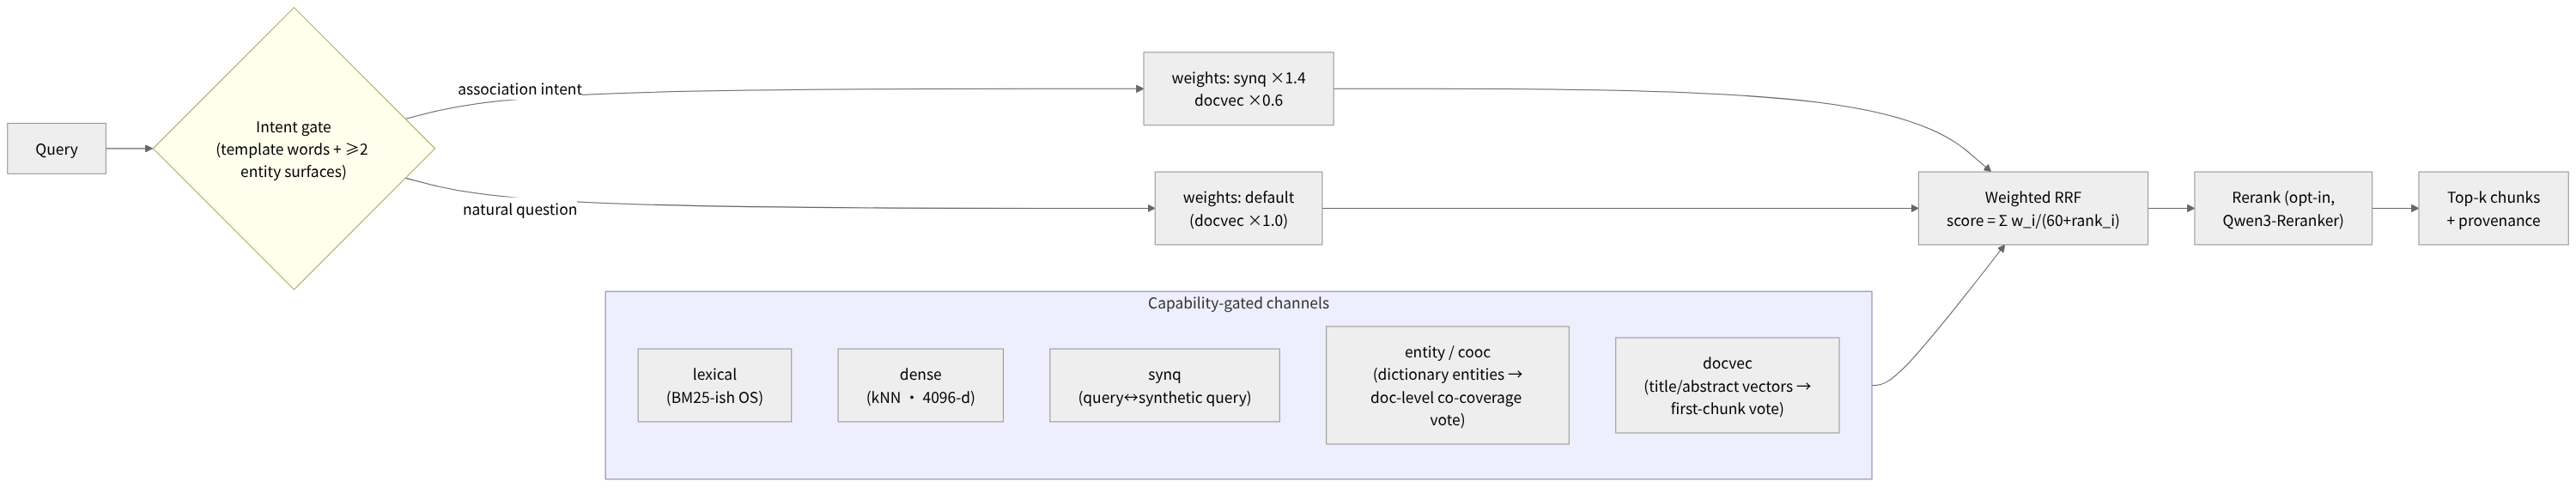
\includegraphics[width=0.92\textwidth]{fig2.png}
\caption{Retrieval planner: capability-gated channels fused by weighted RRF
with intent gating.}
\label{fig:planner}
\end{figure}

\begin{itemize}
\item \textbf{Lexical}: OpenSearch BM25 over chunk text with schema term
boosts.
\item \textbf{Dense}: kNN over chunk vectors (Qwen3-Embedding-8B;
1{,}024-d Matryoshka-truncated on both index and query sides, native
4{,}096-d; HNSW).
\item \textbf{Synq}: kNN over synthetic queries (doc2query, ${\sim}3$ per
chunk, 18{,}454 for the test corpus) matched against the user query vector.
\item \textbf{Entity/Cooc}: dictionary-driven entity mentions $\to$
document-level entity co-coverage vote (intent-gated: template words +
$\geq$2 entity surfaces).
\item \textbf{Docvec} (B84): kNN over title/abstract vectors $\to$
first-chunk proxy vote.
\end{itemize}

\subsection{Intent-gated channel weighting}

We observe that static equal weights are sub-optimal in a domain-dependent
manner (Table~\ref{tab:weighting}).

\begin{table}[t]
\centering
\caption{Intent-gated channel weighting (B83--B85).}
\label{tab:weighting}
\small
\begin{tabularx}{\textwidth}{lXXl}
\toprule
Variant & nea (assoc.) & ner (real) & Verdict \\
\midrule
synq $\times$1.4 global & +4.2pt R@10 & $\mathbf{-7.7}$pt & rejected \\
synq $\times$1.4 intent-gated & +2pt & unchanged & adopted \\
docvec full & +2pt & \textbf{+5pt R@10, +6pt MRR} & adopted \\
docvec assoc-downweight 0.6 & +2pt retained & +5pt retained & adopted \\
lexical $\times$0.3 English non-assoc & (nea unaffected) & (bench +5--17pt) & adopted \\
\bottomrule
\end{tabularx}
\end{table}

The intent gate (template-word regex + $\geq$2 dictionary entity surfaces) is
deliberately lightweight (zero LLM calls) and reproducible across domains:
Chinese association templates (同时涉及/关联检索) and English equivalents
(research both / intersection of) trigger the same reweighting path.

\textbf{Gate validity (confusion analysis, two domains).} Because routing
heuristics that key on named entities are known to over-trigger on multi-hop
queries, we quantify the gate directly against question-set labels
(association sets = positive, real-query sets = negative;
\texttt{gate\_eval.py}, predicates byte-identical to the service). On the
nuclear-electronics set (48 positive / 39 negative), the double gate
(template $\wedge$ $\geq$2 surfaces) attains precision 1.000 / recall 0.854 /
F1 0.921; the entity-surface gate alone attains precision 0.562 (32/39
over-triggered). On a site-contamination set (34/31) the double gate is
perfect (P/R/F1 = 1.000). The template-word stage is what prevents the
documented over-routing failure mode: the entity gate alone fires on
82--97\% of natural queries in both domains. All 7 residual false negatives
are dictionary-coverage gaps (non-entity concepts), not gate-logic errors.
The English non-assoc gate (B85) triggers on 98.5\% of 600 benchmark queries
with a 2.3\% false-trigger rate on Chinese sets. Sample sizes are small (48/39 and 34/31 labelled
questions): the perfect cells are point estimates on tens of
questions---the Wilson 95\% CI for csh recall (34/34) is [0.90, 1.00]---and
we read 1.000 as ``no error observed in-sample'', not as an error bound.

\subsection{The fusion-versus-dense finding}

Across five independent experiments (three English benchmarks + two Chinese
question sets), multi-channel fusion with equal weights underperforms the
dense channel alone on English multi-hop tasks while outperforming it on
Chinese domain queries (Table~\ref{tab:fusiondense}).

\begin{table}[t]
\centering
\caption{Fusion minus dense channel, five experiments.}
\label{tab:fusiondense}
\begin{tabular}{llll}
\toprule
Domain & R@10 diff & MRR diff & Significance \\
\midrule
HotpotQA (full) & $-$0.7pt & $-$1.1pt & n=1000 \\
2Wiki (full) & $-$0.7pt & $-$1.4pt & n=1000 \\
MuSiQue (full) & $-$5.1pt & $-$3.6pt & n=1000 \\
ne association & +2pt & +14pt & CI excludes 0 \\
ne real queries & $-$3pt & +3pt & CI includes 0 \\
\bottomrule
\end{tabular}
\end{table}

This is a \textbf{language/domain dependence} finding, not a general
anti-fusion result: the lexical vote drags English multi-hop rankings (where
BM25 already achieves 85--95\% of dense recall), while on Chinese domain
queries the synq and co-occurrence channels provide genuinely complementary
signal (evidence: synq-only hits 4 questions dense misses on nea). The
per-domain gate is the design response, not the removal of channels.

\subsection{Evaluation methodology}

All ablations use: identical corpus (isolated test stack), identical embedder
(Qwen3-Embedding-8B), identical question sets, paired bootstrap 95\% CI, and
two complementary metrics: any-hit@k (the harness convention, saturated for
small corpora) and cov@k $=$ $|\mathrm{gold} \cap \mathrm{top}\text{-}k| /
|\mathrm{gold}|$ (the set-recall metric that discriminates multi-gold
questions). RRF configuration changes require explicit cache invalidation
(documented after it invalidated results twice).

\textbf{Cluster-robust significance.} Queries generated from the same corpus
are not independent, so per-query bootstrap CIs understate variance when sets
are pooled. We therefore report every pooled comparison under two concurrent
standards: per-query bootstrap CI, and a cluster-level interval over query
sets (cluster bootstrap for $k\geq5$ clusters; cluster-mean t interval for
$k<5$, since the bootstrap degenerates to a $k^k$-point discrete distribution
there and would inflate significance). Cluster-level significance requires
all cluster means to share sign \emph{and} the interval to exclude zero.
Under this discipline the synq+cooc channel gain survives: pooled over four
question sets (two domains, n=152), R@10 +0.250---per-query CI [0.184,
0.322], cluster t CI [0.059, 0.437], all four cluster means positive.
Effects measured on two domains only (e.g.\ the docvec channel,
+2.1/+5.1pt, sign-consistent across both sets) are reported with the explicit
caveat that cluster-robust confirmation needs more domains.

\textbf{Multiple comparisons.} The campaign reports on the order of forty
paired comparisons. We do not apply a family-wise or Benjamini--Hochberg
correction across that family; at the 95\% level roughly two nominally
significant results would be expected by chance alone, and we ask the
reader to weight accordingly: single-CI findings are treated as
suggestive, while corroborated findings---cluster-robust, sign-consistent
across independent question families, or mechanistically attributed
(e.g.\ the failure autopsies below)---carry the paper's claims.

\subsection{Failure attribution: where missed golds are lost}
\label{sec:autopsy}

A channel-isolated autopsy of every missed gold document (97 on nea, 71 on
ner) locates the failing layer: each of the four channels is probed directly
at the engine level (top-100, bypassing the service's channel mixing) and
cross-referenced against the fused ranking (Table~\ref{tab:loss}).

\begin{table}[t]
\centering
\caption{Loss-layer attribution of missed gold documents.}
\label{tab:loss}
\begin{tabular}{lll}
\toprule
Loss layer & nea (n=97) & ner (n=71) \\
\midrule
fused@20 near-miss (rank 11--20) & 33\% & 27\% \\
\textbf{ch@100 dilution} (gold in $\geq$1 channel & \multirow{2}{*}{\textbf{60\%}} & \multirow{2}{*}{\textbf{70\%}} \\
top-100, absent from fused top-20) & & \\
deep recall miss (no channel top-100) & 7\% & 3\% \\
\bottomrule
\end{tabular}
\end{table}

\textbf{93--97\% of misses are aggregation/ranking failures, not recall
failures.} The channels find the documents; chunk-level RRF cannot
consolidate document-level support. Smoking-gun case: one missed gold
document is dense-rank-5 (its chunk \#47), synq-rank-31 (chunk \#4), and
docvec-rank-1 (first chunk \#0)---three channels vote for three
\emph{different} chunks of the same document, each vote individually too weak
to surface any chunk into the top-20. The docvec channel (B84) is a
FirstP-style document signal in the MaxP/FirstP family~\cite{maxp}, but its single
first-chunk vote does not merge with votes landing on other chunks.

This attribution extends component-level RAG diagnosis to the
\textbf{fusion layer} and directly motivates doc-aware fusion (per-channel
per-document best-k vote consolidation before RRF---O10), which targets the
dominant loss layer. Dictionary/enrichment coverage gaps are real but
secondary.

\textbf{Constructive validation on a hard-target set.} We instrument the
dilution layer as a question-set constraint: 37 questions drafted from
non-abstract passages with lexical detachment ($\leq$15\% 8-gram copy rate)
and accepted only if the gold is visible in some channel's top-100 yet
absent from the fused top-10. \textbf{This is a mechanism probe on a
purpose-built adverse distribution, not a representative benchmark}:
questions were selected precisely because the deployed base endpoint fails
them (acceptance rate 6.2\% over 600 drafts on the full production corpus),
so absolute numbers on this set quantify the recovery mechanism
(displacement and its repair), not general retrieval quality.
On this distribution the dilution phenomenon reproduces constructively:
single-dense retrieval already ranks 37.8\% of golds into top-10 (MRR 0.167)
while the fused base endpoint returns 0.000---multi-channel voting displaces
strong single-channel signals on lexically-detached phrasing. BM25 collapses
to zero on all metrics (the detachment gate seals the lexical path by
design). The deep endpoint recovers 62.2\% into top-10 (binomial 95\% CI
[0.45, 0.77], median recovered rank 1). Component separation on the same
set: removing the cross-encoder rerank drops hit@10 from 0.57 to 0.16
(rerank dominates recovery); the PPR graph expansion adds a positive but
modest +2.7pt (37/37 queries fire, p50 +1.9\,s). Together with the
90\%-edge-deletion result (Section~\ref{sec:eng}), this yields the paper's
positioning of graph structure: \textbf{graph assets empower the vector
hybrid} (dictionary $\to$ intent gating and seeding; bilingual aliases $\to$
+7.6pt real-query cov@20; entity-link co-occurrence $\to$ the
association-channel gains), while structural traversal contributes only at
the margin and only inside the budget-constrained deep lane.

\textbf{Doc-aware fusion (O10, adopted).} The fusion re-ranks its candidate
pool by document: doc score $=$ sum of the document's top-$\lambda$ chunk
votes (a truncated-sum variant of the MaxP/SumP family~\cite{maxp}), emitting at most
$\lambda$ chunks per document. The $\lambda$ sweep traces a clean
any-hit/coverage frontier: $\lambda$=1 lifts cov@20 (+5.0pt, per-query CI
significant) with zero @10 change; \textbf{$\lambda$=2 lifts cov@10 +6.28pt
under both CI standards (cluster-t interval [0.029, 0.097], both clusters
positive---the first technique in this campaign to pass cluster-robust
significance; k=2 clusters, so the interval is fragile and the claim is
campaign-scoped, not field-level)} at $-$4.6pt any-hit; $\lambda$=3
overshoots (cov@20 turns
negative). Because the trade is intent-shaped---association queries want
complete coverage, real queries want fast any-hit---the adopted configuration
gates $\lambda$=2 on the association intent: association queries gain the
full coverage lift (cov@10 0.569$\to$0.633), real queries are bitwise
unchanged. The smoking-gun case above now resolves: the three scattered
votes consolidate into a top-ranked document.

\section{NuclearIR-Bench}
\label{sec:bench}

\subsection{Design}

Question sets are generated corpus-first: entity-pair mining from
canonical-entity $\times$ entity-link co-occurrence (gold $=$ documents
covering both entities, 2--6 per pair) $\to$ LLM phrasing in Chinese with
English entity terms preserved $\to$ verification (dedup, gold non-empty).
Three question types are stratified: \textbf{Association} (nea, ``有哪些研究同时涉及X与Y''
---multi-gold by construction); \textbf{Real queries} (ner, natural-language
questions from actual usage logs); \textbf{Title lookups} (net, exact title
retrieval; saturating control).

\subsection{Multi-disciplinary generality}

\begin{table}[t]
\centering
\caption{Multi-disciplinary generality.}
\label{tab:generality}
\begin{tabular}{llll}
\toprule
Domain & KB size (ACTIVE) & Questions & R@10 \\
\midrule
Hydrogeology & 27 docs & 34 (LLM draft) & 0.912 \\
Site contamination & 723 docs & 31 real / 34 assoc & 0.903 / 1.000 \\
Fundamental physics & 1{,}324 docs & 24 & 1.000 \\
Nuclear electronics & 3{,}479 docs & 39 real / 48 assoc & 0.897 / 1.000 \\
\bottomrule
\end{tabular}
\end{table}

Four disciplines, 129$\times$ scale range, all R@10~$\geq$~0.90
(Table~\ref{tab:generality})---corpus-first generation methodology and
retrieval system are domain-general.

\subsection{Benchmark validity controls}

Two controls establish that the question sets measure retrieval rather than
artifact (\textbf{closed-book}) and that cov@k is interpretable as a
conservative lower bound (\textbf{unjudged audit}):

\begin{enumerate}
\item \textbf{Closed-book control} (HybridRAG-Bench protocol): asking the LLM
directly which papers answer each question---without retrieval---yields a
gold-document naming rate of \textbf{0/48 (nea) and 0/39 (ner)} (86/87
answers are ``don't know''). The gold documents are domain journal papers
unseen in pretraining; the benchmark cannot be solved from model memory.

\item \textbf{Unjudged audit} (topic-specific re-judging): we re-judge a
sample of top-10 retrieved but unjudged (non-gold) documents under a strict
evidence-quotation protocol---the judge receives each entity's full
bilingual name set (canonical + aliases) and must quote one passage of
original text per entity side; a ``relevant'' verdict additionally requires
programmatic verification that both quotes are present in the document.
Result: 18/203 sampled unjudged documents on nea carry verified both-entity
evidence---cov@10 is a conservative lower bound with \textbf{correction
$\leq$+8.1pt (nea) and $\leq$+2.4pt (ner)}. A naive one-word relevance
protocol over-estimates the correction 3$\times$ (+24.7pt) and is falsified
by a surface cross-check (0/76 of its ``relevant'' verdicts have both entity
surfaces in the document)---we report this as a measurement methodology
finding: unjudged re-judging without entity name sets and verifiable quotes
is not trustworthy.

\item \textbf{Generation circularity (acknowledged and bounded).} The
association question sets are generated from the same entity-pair
co-occurrence assets that the co-occurrence channel consumes---the gold
criterion (documents covering both entities) coincides with the channel's
mechanism, so association-set numbers partially measure the asset they
were built from. We bound rather than deny this: (a)~the closed-book
control above rules out memorization, not circularity; (b)~the
natural-phrasing variants (template words banned) still show the
co-occurrence channel's +10.1pt hit@10 gain (CI [+5.1, +16.2]; distinct
from the query-time-LLM pipeline's +10.1pt cov@10 in the capability
comparison, a numbering coincidence)---the channel works through
dictionary-surface hits in the query, not template-word leakage; (c)~single-intent real queries define
gold by information need with no entity-pair construction; and (d)~the
English public benchmarks involve none of our assets. Additionally, a
single-variable channel ablation on the scoped association set under the
final configuration shows the entity-dependent channels contribute
bitwise-zero to fused ranking there (next section)---the benchmark is not
being carried by the entity machinery it was generated from, at least at
the fusion layer. Corpus-construction-level claims (bilingual aliases,
dictionary coverage) remain partially circular, and we label them as such
where they appear.
\end{enumerate}

\section{Results}
\label{sec:results}

\subsection{Full-corpus benchmark comparison}

On the HippoRAG~2 evaluation protocol (1{,}000 queries $\times$ full
candidate corpora, R@2/R@5; Table~\ref{tab:bench}):

\begin{table}[t]
\centering
\caption{Full-corpus benchmark comparison (R@2/R@5).}
\label{tab:bench}
\begin{tabular}{lllll}
\toprule
Method & HotpotQA & 2Wiki & MuSiQue & Embedder \\
\midrule
BM25 & 57.3/74.8 & 55.3/65.3 & 32.4/43.5 & --- \\
NV-Embed-v2 & 84.1/94.5 & 67.1/76.5 & 52.7/69.7 & NV-Embed-v2 \\
HippoRAG 2 & 83.5/96.3 & 76.2/90.4 & 56.1/74.7 & NV-Embed-v2 \\
\textbf{KNC dense} & \textbf{94.6/97.4} & \textbf{99.7/99.9} & \textbf{85.7/91.2} & Qwen3-Emb-8B \\
KNC fusion & 93.9/97.9 & 99.0/100.0 & 80.6/91.3 & Qwen3-Emb-8B \\
\bottomrule
\end{tabular}
\end{table}

\textbf{This table is an embedder-generation comparison, not an
architecture comparison}: KNC-dense and the NV-Embed-v2 rows differ in
both system and embedding model (Qwen3-Embedding-8B, 2025, versus
NV-Embed-v2, 2024), so the +10--30pt gap cannot be attributed to
infrastructure. To separate the two factors we re-ran the systems
\textbf{under the same embedder} (all Qwen3-Embedding-8B, identical
stack and scoring, 400-document pools with 40/46/23 questions per
benchmark; Table~\ref{tab:bench-sameemb}).

\begin{table}[t]
\centering
\caption{Same-embedder control (cov@10; all arms Qwen3-Embedding-8B,
400-doc pools).}
\label{tab:bench-sameemb}
\begin{tabular}{llll}
\toprule
System & HotpotQA & 2Wiki & MuSiQue \\
\midrule
BM25 & 0.888 & 0.766 & 0.467 \\
LlamaIndex dense & 0.963 & 0.772 & 0.732 \\
\textbf{HippoRAG 2 (reproduced)} & \textbf{1.000} & \textbf{0.913} & 0.779 \\
KNC dense & 0.988 & 0.826 & \textbf{0.826} \\
KNC fusion & 0.975 & 0.794 & 0.656 \\
\bottomrule
\end{tabular}
\end{table}

The same-embedder control \textbf{reverses the reading}: HippoRAG~2's
graph machinery outperforms plain dense retrieval on 2 of 3 benchmarks
(2Wiki +8.7pt, HotpotQA +1.2pt over KNC-dense) and trails on MuSiQue
($-$4.7pt)---at pool scale its structure pays where multi-hop
composition dominates. What KNC adds on these English benchmarks is not
fusion (KNC fusion $\leq$ KNC dense everywhere here, consistent with
the ungated-fusion degradation of Section~\ref{sec:channels}) but the
operational substrate (production indexing, scale, traceability); the
domain-side advantage story lives in the nuclear-electronics sections,
not here. We report the reversal against interest: architecture claims
in Table~\ref{tab:bench} belong to the embedding model, not to us.

\subsection{Controlled ablation on the nuclear-electronics domain}

Post-rebuild refresh (2026-10-09): after the schema-lexicon repair
(Section~\ref{sec:incident}) the scoped arms were re-run under the
production-final configuration---associative queries cov@10
0.533$\to$\textbf{0.599}, single-intent 0.603$\to$\textbf{0.675}, MRR
$-$2.0/+5.0pt against the pre-rebuild baseline. The trajectory is
system-level (two weeks of retrieval configuration evolution plus the
lexicon repair); we bound it with a single-variable channel ablation under
the identical final configuration---all entity-dependent channels off
(co-occurrence, graph, entity-vector, PPR) versus the full stack:
\textbf{metrics are bitwise identical on both families} (cov@10/R@10/MRR
unchanged; the only movement is associative cov@20 $-$1.0pt, 95\% CI
[$-$3.1, 0.0]) while p50 latency halves (1.46\,s $\to$ 0.52\,s). Two
readings follow. First, the repair-window trajectory above is carried by
the non-entity configuration evolution, not by entity channels casting
fusion votes---we state this against interest. Second, on these benchmark
families the entity layer's retrieval-facing value does not run through
fusion at all: it runs through lexical alias expansion (entity names as
BM25 terms), deep-lane reranker context, and generation-side knowledge
chains---consistent with the graph-governance nulls reported later in
this section.

\textbf{Channel $\times$ question-distribution contribution matrix.} The
apparent contradiction between this zero-effect result and the channel
gains reported elsewhere resolves once the distribution axis is made
explicit:

\begin{table}[t]
\centering
\caption{Where the entity channels pay: contribution by question
distribution.}
\label{tab:channmatrix}
\small
\begin{tabularx}{\textwidth}{lXXXX}
\toprule
Distribution & co-occ. & graph/PPR & entity-vec & synq \\
\midrule
nea48/ner39 scoped, final config & 0 (fired 6/48, all ties) & 0 (bridge-only) & 0 (no candidates) & $>$0 (4 Qs) \\
99 natural-phrasing assoc & hit@10 \textbf{+10.1} [+5.1,+16.2] & --- & --- & --- \\
hard37 probe, deep lane & --- & PPR \textbf{+2.7pt} & --- & --- \\
English multi-hop pools & n/a & n/a & n/a & $\leq$0 \\
Pooled 4 sets, earlier config & \multicolumn{4}{l}{synq+cooc R@10 +0.25, cluster-robust} \\
\bottomrule
\end{tabularx}
\end{table}

The mechanism behind the bitwise identity on the scoped sets is
fourfold, not mysterious: (a)~the co-occurrence channel's adaptive gate
fires only when base-retrieval heads do \emph{not} already serve
co-mention documents---under the final configuration (alias expansion +
doc-fusion) they do, on 42/48 questions, so the channel self-extinguishes
(its designed behaviour, not a bug); (b)~the graph channel is an
output-surface channel: it appends bridge chains only when their
endpoints do \emph{not} co-occur in the returned chunks, and casts no RRF
votes; (c)~the entity-vector channel produced no candidate chunks in this
configuration; (d)~PPR is gated to the deep lane. Removing channels that
cast no votes removes nothing---which is also why the same removal
\emph{does} cost on distributions where the gates open
(Table~\ref{tab:channmatrix}: +10.1pt row 2, +2.7pt row 3).

\textbf{Why they ship enabled.} The operations answer, stated as such:
(1)~the benchmark families under-represent the traffic the channels
insure against---naturally-phrased association queries are real usage
(the 99-question set exists because of them) and hard queries recover via
deep-lane PPR (+2.7pt); (2)~the graph channel serves the evidence surface
(knowledge chains in output) regardless of ranking; (3)~the deep lane
consumes entity assets (reranker context, chain evidence for
generation); (4)~p50 1.46\,s sits inside the deployed SLO with the
channels on. A latency-first deployment could gate the normal lane's
entity channels off at zero measured benchmark cost---a configuration
decision the ablation makes available, not a necessity claim we retreat
from.

\subsection{Scale curve}

At 16$\times$ corpus growth (300$\to$4{,}850 docs), the dense baseline drops
from 95.8\% to 62.5\% any-hit@10 while KNC full-channel maintains 100\%;
coverage@10: KNC 0.669 versus baseline 0.351 (+32pt). Latency: KNC 1.3\,s
versus 35.9\,s for the dense baseline---a LlamaIndex retriever without an
ANN index, which degenerates to a brute-force scan over the 196k-chunk /
37\,GB vector store at this scale; the latency gap is thus an artifact of
the baseline's deployment mode, and we read it as ``a production-grade
index is necessary at this scale'', not as a 27$\times$ algorithmic
advantage.

Post-rebuild full-scale tier (80{,}852-document production,
${\sim}$250$\times$ the slice): associative queries any-hit@10
\textbf{1.000}, cov@10 0.652, MRR 0.624, p50 1.46\,s; single-intent any-hit
0.923, cov@10 0.600, p50 1.46\,s. Coverage holds within noise of the
4{,}850-document tier (0.669$\to$0.652) and latency does not move---under
the fused, intent-gated architecture the scale cliff observed in
single-vector baselines does not appear through 250$\times$ growth. The
scoped-slice versus full-library comparison under identical questions shows
the filter-restricted slice is the \emph{harder} condition for associative
queries (0.599 versus 0.652) and the easier one for single-intent (0.675
versus 0.600): distractor mass and candidate restriction act in opposite
directions by query type. No external baseline ran at this
250$\times$ tier---the full-library numbers are system telemetry on the
production corpus, and all baseline comparisons in this paper live at the
300- and 4{,}850-document tiers.

\subsection{Domain-specific comparison}

LightRAG (13\,h construction) ranks last on nuclear electronics (cov@10
0.471 versus KNC 0.667) while competing on English benchmarks---LLM-extracted
entities fail on domain-specific terminology (10.6\% chunk NER failure rate
on nuclear full text versus 0.25\% on Wikipedia).

\subsection{Construction cost}

\begin{table}[t]
\centering
\caption{Construction cost.}
\label{tab:cost}
\small
\begin{tabularx}{\textwidth}{lXXl}
\toprule
System & ne 300 docs & Benchmark 400 docs & Bottleneck \\
\midrule
KNC enrichment & ${\sim}$1\,h & ${\sim}$2\,min & synq doc2query (LLM) \\
HippoRAG 2 & 4.1\,h & 13--14\,s (warm) / 40\,min (cold) & OpenIE (LLM) \\
LightRAG & $>$13\,h (82 docs only) & infeasible & entity merge (serial CPU) \\
\bottomrule
\end{tabularx}
\end{table}

Table~\ref{tab:cost} summarises: KNC construction costs 1--2 orders of
magnitude less than graph-RAG alternatives at domain scale. The cost comparison is \textbf{asymmetric by design and we say so}:
LightRAG and HippoRAG~2 pay per-chunk LLM extraction at construction,
our K1 is a dictionary scan---the table prices two different design
points of entity acquisition, not the same workload twice. That
asymmetry is the finding: LLM-extraction cost is what blocks graph-RAG
at production scale, and the dictionary design point shifts the quality
burden onto the lexicon (Section~\ref{sec:incident}).

\subsection{Capability pipeline comparison: query-time LLM versus
accumulated assets}

How far can a pure query-time LLM pipeline go on the same corpus,
spending its budget per query instead of at construction? We built a
capability-side arm (``genrag'', 2026-10-07): LLM query rewriting
$\to$ BM25(jieba) + dense(Qwen3-Embedding-8B) fused by RRF $\to$ LLM
list rerank of the top-60 to 20---the ``LLM everywhere at query time''
design point, run on the same scoped questions with identical scoring
(n=48/39, paired bootstrap against the same-day KNC configuration):

\begin{table}[t]
\centering
\caption{Capability pipeline versus asset pipeline (same corpus, same
questions, same day).}
\label{tab:genrag}
\small
\begin{tabularx}{\textwidth}{lXXXXXXX}
\toprule
System & nea R@10 & nea cov & nea MRR & ner R@10 & ner cov & ner MRR & p50 \\
\midrule
genrag (query-time LLM) & 0.896 & \textbf{0.634} & 0.735 & 0.872 & 0.543 & \textbf{0.780} & 79--83\,s \\
KNC (asset side) & 0.917 & 0.560 & 0.715 & 0.949 & \textbf{0.636} & 0.754 & ${\sim}$1.3\,s \\
\bottomrule
\end{tabularx}
\end{table}

The query-time pipeline wins association cov@10 \textbf{+10.1pt (CI
[2.6, 18.4], significant)}---query rewriting genuinely widens the
retrieval surface on multi-gold association questions---and loses
single-intent cov@10 ($-$5.9pt) while paying ${\sim}$60$\times$ latency
(79--83\,s versus 1.3\,s) and 2$\times$N LLM calls per question set with
zero asset accumulation (every query re-pays; every corpus change
re-prices). The KNC position is the complement: assets (aliases, synq,
entity layers) amortize construction cost across queries and keep p50 in
the low seconds. We read this as the capability-versus-infrastructure
trade-off priced from both sides, each winning where its cost structure
fits. (Numbering coincidence, flagged for the careful reader: the
co-occurrence channel's marginal on the natural-phrasing set---
Table~\ref{tab:channmatrix} row~2---is also +10.1pt, on hit@10 with CI
[+5.1, +16.2]; a different experiment.)

\section{Discussion and Limitations}
\label{sec:discussion}

\subsection{Production-scale schema-quality incident and repair}
\label{sec:incident}

Enriching 61{,}137 documents with a \emph{category-word} schema lexicon
collapsed the entity layer to 575 type-level vertices carrying ${\sim}$19.2M
links (``method'', ``energy'' as entities) while every job-level monitor
stayed green. A three-source, corpus-attested term lexicon (3{,}702 entries)
and a full-chain rebuild restored it to 1{,}871 canonical entities with
25.1M links and a functioning relation layer (44{,}043 typed relations, 1.56M
evidence rows); scoped retrieval over the repair window moved +6.6/+7.3
cov@10 (system-level attribution, Section~\ref{sec:results}). Two honest
boundaries: the top-linked entities after repair remain generic short
symbols (admission without ranking), and the repair itself surfaced four
secondary engineering failures---most instructively a parameter-order bug
whose rows were silently swallowed by \texttt{INSERT IGNORE} for seven hours
while jobs, throughput, and entity creation all read healthy. Dictionary
quality is the load-bearing wall of dictionary-driven extraction; job
completion is not row-level truth. The full incident forensics and lexicon
methodology are reported in the companion lexicon-quality manuscript.

\subsection{Negative results (with equal rigour to positive ones)}

\textit{Naming convention: findings carry internal workstream codes
(B4x--B9x, O-serials, and \texttt{KNC\_*}/\texttt{RRF\_*} environment
gates) verbatim, because those identifiers are the join keys into the
released evaluation log and repository history; they name no external
systems.}
\label{sec:negative}

\begin{enumerate}
\item \textbf{Reranker.} After fixing the gateway bug (thinking-tag prefix
removal) and a control-flow bug (reranked chunks overwritten by RRF),
rerank still showed no significant gain (nea MRR +0.9pt, CI includes 0; p50
+2.8\,s). The top-60 candidates from fusion are already consensus; the
bottleneck is recall (cov@k), not ranking.

\item \textbf{Doc caps} (RRF\_DOC\_CAP=2): improved multi-gold association
coverage but degraded single-gold MRR by 11pt---a structural trade-off, not
a bug.

\item \textbf{Static channel weights}: rejected on the principle that fusion
gains are query-type-dependent; intent gating is the only viable path.

\item \textbf{Document-utility priors} (O8): per-document prior conditioning
of the docvec vote (recency decay via \texttt{publish\_year}, injected as an
entry-level multiplier in the rank fusion) was ablated with real publication
years back-filled for 169/300 slice documents (2017--2026). The prior moves
nea and ner in opposite directions on the two metrics; the gain--loss
frontier is linear on both sides---a linear trade, not a tunable shape.
Failure attribution: training-free abstracts are ``too fluent''---they match
topically adjacent non-gold abstracts as strongly as gold, while the gold
criterion is entity-pair co-occurrence, not topical adjacency. The
deep-lane rewrite slot remains open for trained rewriters; the mechanism
stays env-gated for reuse.

\item \textbf{Query-side augmentation family} (equal-rigour rejections): LLM
multi-query fan-out with uniform RRF is significantly negative under the
adopted configuration (nea R@10 $-$8.3pt, MRR $-$20.5pt; ner R@10
$-$10.3pt---per-query CI excludes zero) though positive (+8.4pt cov@10)
under weak fusion---i.e.\ the literature's fan-out gains apply to weak
retrievers and are pre-empted by tuned fusion; pointwise reranking of the
top-20 candidates is significantly harmful on multi-gold questions (MRR
$-$37.7pt: partially-relevant golds score below multi-channel consensus);
listwise LLM reranking is statistically flat. A frozen 261-question
paraphrase-robustness set shows the system is already phrasing-stable
(hit@10 retention 96.5\%/88.9\%), explaining why query-side gains have
nothing left to buy.

\item \textbf{Channel fetch depth} (O12): association-intent depth tripling
gains +4.0pt cov@10 (significant) on the 300-doc slice but $-$2.6pt
(non-significant, negative) at full-corpus scale---weak-ticket interference
grows super-linearly with corpus size. Rolled back to depth 1;
slice-significant $\neq$ corpus-significant is itself a reported finding.

\item \textbf{Generation-side context organisation}: sentence-level
query-aware pruning of the retrieved context yields +6.0/+3.3pt
answer-correctness directionally over two rounds (n=39/87, ns) and a
significant +1.8pt faithfulness on the 87-question round; document-card
headers help relevancy only; combining both mechanisms interferes
($-$5.1pt). Conditioning the pruner on question type is future work.

\item \textbf{Graph-side governance and bipartite diffusion}: motivated by
graph-asset audits (87\% of entity--relation edges are bibliographic
authorship stars; the doc--entity bipartite with 1.37M links is the densest
asset), three mechanisms were ablated against the deployed deep lane:
(a)~typed-edge governance of PPR (excluding/downweighting authored-by and
affiliated-with edges, with bibliographic seed-type guards), (b)~dense
entity-linking fallback for seeds when the lexicon scan misses, and
(c)~a doc-level bipartite PPR channel. Mechanism-level checks confirm the
interventions changed walk behaviour (person-seeded expansions drop
31$\to$0 entities). Outcome: (a)+(b) are bitwise identical to baseline on
every question---PPR's total contribution (${\sim}$1 question) sits below
the deep lane's sensitivity floor; (c) is significantly negative (nea hit@10
$-$4.2pt, CI excludes zero; hard-set $-$2.2pt; p50 +7\,s): the bipartite
asset's value is already captured by the cooc channel's exact entity-pair
intersection, and soft generalisation only dilutes fusion. All remain
env/request-gated and disabled---the asset-layer positioning of graphs gains
a sixth independent line of evidence.

\item \textbf{LLM query understanding on the deep lane}: a single LLM call
per deep request classifies intent and extracts entity surfaces, overriding
the template-word intent gate (natural-phrasing coverage 4/70) and feeding
co-occurrence candidates. Verdict quality is high (48/48 template-assoc
correctly labelled), yet on the target distribution of naturally-phrased
association questions the hit count is unchanged (0 wins, 0 losses; MRR
$-$0.04) and hard factual questions lose 2.2pt from assoc-mechanism false
triggers: the bottleneck for natural association queries is not intent
detection---the association machinery itself buys nothing there. Rejected;
the understanding slot stays available for trained rewriters.

\item \textbf{Deep-lane weight retune and graph-aware reranking} (both
\textbf{ADOPTED}): single-variable attribution over the production tuning
bundle shows the title-vector (docvec) channel actively harms the deep lane
on both question families---its votes push co-occurrence winners out of the
fusion pool, which reranking cannot recover (nea hit@20 $-$4.2pt, hard-set
hit@10 $-$3.2pt); the doc-fusion step is the sole source of the hard-set
hit@20 gain and alias expansion is strongly positive, so both stay.
Complementarily, appending each candidate's top linked document entities
(mention-count top-8) to the reranker input lets graph assets reach the
ranking surface directly, bypassing RRF dilution---the first positive
graph-side mechanism of the campaign. The deployed combination (deep lane
drops docvec and the synq boost; rerank inputs carry document entities)
improves every metric on both families---nea 0.896/0.917/0.583 $\to$
0.958/1.000/0.767 (hit@10/hit@20/MRR, hit@20 saturated), hard-set
0.527/0.634/0.380 $\to$ 0.591/0.645/0.429---with 4 of 6 metrics significant
under paired bootstrap and no negative metric. The normal lane keeps its
own tuned configuration: per-lane weights are precisely what the dual-track
design is for.

\item \textbf{Asset-layer completions and the generation-side path}:
query-mined dictionary backfill adds 246 corpus-verified concepts (PWR
df=88, nuclear physics df=175---core terms previously absent), taking
template-association hit@10 to a saturated 1.000 (48/48) while
natural-phrasing co-occurrence coverage grows 50\%; alias expansion (749
validated entries) is retained as a no-cost asset. A latent budget bug
(the deep lane's 120\,s deadline was frozen at import time, so graph/cooc
channels were silently skipped under load) is fixed and the graph channel
genuinely serves deep requests again. With chains live, injecting
knowledge-chain evidence into the generation context yields correctness
+0.25 (CI [+0.021, +0.521], n=48)---the first significant positive result
for structural graph evidence, completing the positioning: asset layer feeds
retrieval, structural layer feeds generation; graphs need not enter ranking
to pay their way. On a purpose-built 99-question natural-phrasing
association set (template words banned, gold $=$ co-mention documents), the
co-occurrence channel's marginal is +10.1pt hit@10 (CI [+5.1, +16.2], 10
wins 0 losses) over the identical configuration with the channel off---the
asset-layer route's definitive number: template saturated at 1.000, natural
phrasing +10pt at zero cost.
\end{enumerate}

\subsection{Engineering findings}
\label{sec:eng}

\begin{enumerate}
\item \textbf{Filtered HNSW robustness}: 16\% foreign-corpus vectors in a
shared index cause zero steady-state degradation of the dense channel
(measured over 3 days, 98 prediction files). Write-window rank jitter
($\pm$6pt arm-level on borderline questions) is a transient, not a permanent
loss.

\item \textbf{LightRAG scale wall}: single-process entity merging is
superlinear in graph size---82 docs/11.5k chunks/13k+ entities $\to$
${\sim}$1 doc/hour after the first 47 docs. LLM extraction concurrency
(16$\to$70) helps; merge does not.

\item \textbf{Link-edge mass is redundant}: randomly deleting 30/60/90\% of
the 158{,}057 entity links of the test KB causes no statistically
significant retrieval change (nea at 90\% deletion: R@10 $-$2.1pt, cov@10
$-$2.7pt, all CI include zero; ner bitwise unchanged). Edge quality
dominates edge count, and link value anchors in the structural surfaces
(governance, navigation, evidence panels), not in the fusion vote.

\item \textbf{Schema binding is the root of the entity channel}: binding a
corpus to the \texttt{generic} schema yields 14 canonical entities;
rebinding to \texttt{nuclear\_electronics} yields 1{,}166---an 83$\times$
difference with zero code changes, purely from the dictionary.
\end{enumerate}

\subsection{Limitations}

\begin{enumerate}
\item Single-corpus domain (nuclear electronics) for the primary ablation;
English benchmarks provide external validity but not domain depth.
\item Synquestion generation requires LLM access (${\sim}$40 calls per
document for synq + relations); offline corpora need a pre-processing pass.
\item The intent gate is regex-based; LLM-based query classification could
improve coverage but adds latency (SelRoute: 83\% accuracy with regex).
\end{enumerate}

\section*{Data availability}

Question sets (nea/ner, 48+39 questions), evaluation scripts
(paired-bootstrap scoring, scoped runners, the channel-ablation runner),
and the lexicon-generation tooling are released with the repository at
\url{https://devgit.cdut.edu.cn/chenzhiqian/knowledgenexus} (institutional
GitLab; access on request). The journal corpus itself is
third-party copyrighted material; we release document-level metadata
(venue/year/identifier) and chunk-level gold annotations for the evaluation
slices instead. The production incident telemetry in
Section~\ref{sec:incident} is sanitised log excerpts.

\section*{Conflict of interest}

The authors declare no competing interests.

\begin{thebibliography}{16}

\bibitem{fayyaz} Y.~Fayyaz, W.~Elouataoui, et al. Natural language
processing in the nuclear industry: Opportunities and challenges.
\emph{Nuclear Technology}, 2025. doi:10.1080/00295450.2025.2481358.

\bibitem{radiantllm} RADIANT-LLM: An agentic retrieval augmented generation
framework for safety-critical nuclear engineering. arXiv:2604.22755, 2026.

\bibitem{nukelm} D.~Burke, K.~Pazdernik, et al. NukeLM: Pre-trained and
fine-tuned language models for the nuclear and energy domains.
arXiv:2105.12192, 2021.

\bibitem{curielm} CurieLM: Enhancing large language models for nuclear
domain. \emph{EPJ Web of Conferences} 302, 17006, 2024 (SNAMC 2024);
ontology integration in CEUR-WS Vol.~3967.

\bibitem{hydrollm} Toward HydroLLM: A benchmark dataset for
hydrology-specific knowledge assessment for large language models.
\emph{Environmental Data Science}, Cambridge University Press, 2025.

\bibitem{hipporag} B.~J. Guti\'errez et al. HippoRAG: Neurobiologically
inspired long-term memory for large language models. NeurIPS 2024.
arXiv:2405.14831.

\bibitem{hipporag2} HippoRAG 2: From RAG to memory: Non-parametric
continual learning for large language models. ICML 2025. arXiv:2502.14802.

\bibitem{lightrag} LightRAG: Simple and fast retrieval-augmented generation.
arXiv:2410.05779, 2024.

\bibitem{qwen3emb} Qwen3 embedding: Advancing text embedding and reranking
through LLMs. arXiv:2506.05176, 2025.

\bibitem{vllm} W.~Kwon et al. Efficient memory management for large language
model serving with PagedAttention. SOSP 2023. arXiv:2309.06180.

\bibitem{rrf} G.~V. Cormack, C.~L. A. Clarke, S.~Buettcher. Reciprocal rank
fusion outperforms Condorcet and individual rank learning methods.
\emph{Proc. SIGIR}, 2009. doi:10.1145/1571941.1572114.

\bibitem{doc2query} R.~Nogueira, J.~Yang, J.~Lin, K.~Cho. Document
expansion by query prediction. arXiv:1904.08375, 2019.

\bibitem{hyde} L.~Gao, X.~Ma, J.~Lin, J.~Callan. Precise zero-shot dense
retrieval without relevance labels. \emph{Proc. ACL}, 2023.
arXiv:2212.10496.

\bibitem{graphrag} D.~Edge, H.~Trinh, N.~Cheng, et al. From local to
global: A graph RAG approach to query-focused summarization.
arXiv:2404.16130, 2024.

\bibitem{raptor} P.~Sarthi, S.~Abdullah, A.~Raghunathan, et al. RAPTOR:
Recursive abstractive processing for tree-organized retrieval.
\emph{Proc. ICLR}, 2024. arXiv:2401.18059.

\bibitem{maxp} Z.~Dai, J.~Callan. Deeper text understanding for IR with
contextual neural language modeling. \emph{Proc. SIGIR}, 2019.
arXiv:1905.09217.

\end{thebibliography}

\end{document}
